\documentclass[a4paper,12pt,twoside,openright,titlepage]{book}

%Additional packages
\usepackage[utf8]{inputenc}
\usepackage[T1]{fontenc}
\usepackage[dutch,english]{babel}
\usepackage{syntonly}
\usepackage[official]{eurosym}
\usepackage{csquotes}

% Handle images
\usepackage{graphicx}
\graphicspath{ {./images/}{./styles/} }
\usepackage{float}
\usepackage{wrapfig}

% Handle URLs
\usepackage{xurl}
\usepackage{hyperref}
\hypersetup{colorlinks=true, linkcolor=blue, citecolor=blue, filecolor=blue, urlcolor=blue, pdftitle=, pdfauthor=, pdfsubject=, pdfkeywords=}

% Tables and listings
\usepackage{multirow,tabularx}
\usepackage[table]{xcolor} % Table colors
\usepackage{scrextend}
\addtokomafont{labelinglabel}{\sffamily}
\usepackage{listings}
\usepackage{adjustbox}

% Turn on indexing
\usepackage{imakeidx}
\makeindex[intoc]

% Define colors
\usepackage{color}
\definecolor{ashgrey}{rgb}{0.7, 0.75, 0.71}




% Listing style
\lstset{
  backgroundcolor=\color{ashgrey}, % choose the background color; you must add \usepackage{color} or \usepackage{xcolor}; should come as last argument
  rulecolor=\color{black},         % if not set, the frame-color may be changed on line-breaks within not-black text (e.g. comments (green here))
  frame=single,	                   % adds a frame around the code
  basicstyle=\footnotesize\ttfamily,  	   % the size of the fonts that are used for the code
  extendedchars=true,    	   % lets you use non-ASCII characters; for 8-bits encodings only, does not work with UTF-8
  breakatwhitespace=true, 	   % sets if automatic breaks should only happen at whitespace
  breaklines=true,        	   % sets automatic line breaking
  keepspaces=true,        	   % keeps spaces in text, useful for keeping indentation of code (possibly needs columns=flexible)
  columns=fullflexible,	  	   % Make sure no extra spaces are added.
  showstringspaces=false, 	   % if true show spaces in strings adding particular underscores
  showspaces=false        	   % show spaces everywhere adding particular underscores; it overrides 'showstringspaces'
}



% Uncomment for production
% \syntaxonly

% Style
\pagestyle{headings}

% Define document
\author{D. Leeuw}
\title{Python}
\date{\today\\v.0.1.0}

\begin{document}
\selectlanguage{dutch}

\maketitle

\copyright\ 2025 Dennis Leeuw\\

\begin{figure}

\includegraphics[width=0.3\textwidth]{CC-BY-SA-NC.png}
\end{figure}

\bigskip

Dit werk is uitgegeven onder de Creative Commons BY-NC-SA Licentie en laat anderen toe het werk te kopi\"eren, distribueren, vertonen, op te voeren, en om afgeleid materiaal te maken, zolang de auteurs en uitgever worden vermeld als maker van het werk, het werk niet commercieel gebruikt wordt en afgeleide werken onder identieke voorwaarden worden verspreid.


%%%%%%%%%%%%%%%%%%%
%%% Introductie %%%
%%%%%%%%%%%%%%%%%%%

\frontmatter
\chapter{Over dit Document}
%\input{src/OverDitDocument}
%\input{src/DocChanges_Server}

%%%%%%%%%%%%%%%%%
%%% De inhoud %%%
%%%%%%%%%%%%%%%%%
\tableofcontents

\mainmatter
% requires: 
% provides: programmeren, python
\chapter{Wat is Python?}
Python is een programmeertaal\index{programmeertaal}. Met een programmeertaal kan je een computer dingen voor je laten doen. Doordat de computer dan werk voor je doet kan jij andere dingen doen (nee, niet gamen). Tijdens het programmeren\index{programmeren} gebruik je een programmeertaal om programma-code\index{programma-code} of kortweg code\index{code} te schrijven. De programma-code schrijf je in een tekst-bestand zonder opmaak, we gebruiken daarom geen Word om een computer programma te schrijven maar een editor\index{editor}. Een editor is een heel simpele tekstverwerker zonder alle speciale functies als het invoegen van plaatjes, het nummeren van pagina's of het maken van hoofdstuk-koppen. De meeste programmeurs gebruiken een IDE\index{IDE} (Integrated Development Environment\index{Integrated Development Environment}).

Er zijn verschillende talen om een computer te vertellen wat hij moet doen. Python is er daar \'e\'en van. Programmeertalen kunnen grofweg in twee soorten verdeeld worden. We hebben de scripting-talen\index{scripting} en de talen die eerst gecompileerd\index{gecompileerd} moeten worden.

Talen die eerst gecompileerd moeten worden worden ook geschreven in een editor of een IDE, maar nadat het programma geschreven is gaat deze eerst door een compiler\index{compiler}. Deze compiler maakt van de programma-code een binary\index{binary}. Op Windows systemen is dit vaak een bestand met de extensie .exe van executable\index{executable}. Een executable is een programma dat direct door een computer uitgevoerd kan worden. De binary bevat 1-en en 0-en die direct door de computer begrepen worden. Een executable kan dan ook op elke computer, met dezelfde processor en hetzelfde operating system, uitgevoerd worden zonder dat de programma-code aanwezig is.

Scripting talen hebben geen compiler, maar een interpreter\index{interpreter}. De taal waarin het programma is geschreven wordt op de computer door de interpreter omgezet naar machinetaal\index{machinetaal}, of wel de 1-en en 0-en, om dan uitgevoerd te worden. Op elke computer waarop je het programma wilt draaien moet dus een interpreter en de code aanwezig zijn om de code te kunnen uitvoeren.

Python is een scriptingtaal en heeft dus een Python-interpreter nodig om gebruikt te kunnen worden.

\section{Opdrachten}
\begin{enumerate}
\item Zoek op Internet naar 3 programmeertalen die gecompileerd moeten worden en welke compiler daarvoor gebruikt kan worden
\item Zoek op Internet naar 3 programmeertalen die net als Python ook scripting-talen zijn en welke interpreter daarvoor nodig is
\item Zijn compilers en interpreters binaries? Leg je antwoord uit.
\end{enumerate}

\section{Installatie van de Python-interpreter}
\subsection{Windows}
Volg de instructies op \url{https://learn.microsoft.com/en-us/windows/python/scripting} om Python te installeren. Alleen het kopje \textquote{Install Python}. Je installeert nu de Python-interpreter.

Als Python ge\"installeerd is kan je via de zoekbalk Python opzoeken en opstarten, zoals je kan zien in \ref{fig:pythonint}

\begin{figure}[H]
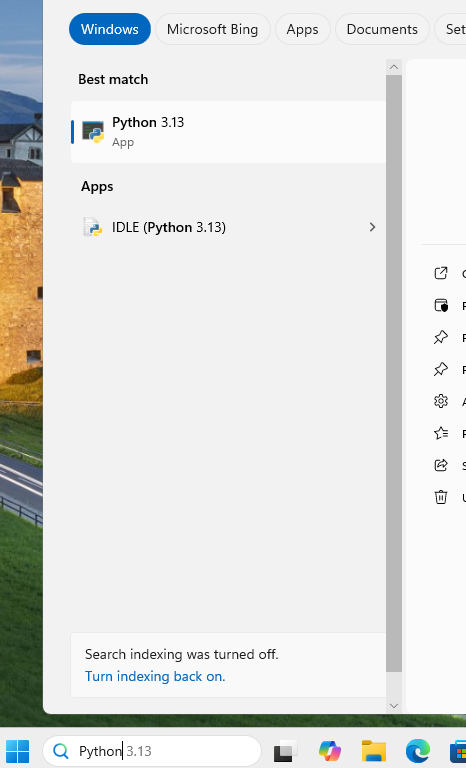
\includegraphics[width=0.9\textwidth]{Screenshot-Python-Start-Selection.png}
        \caption{Zoek en start Python}
        \label{fig:pythonint}
\end{figure}

Om de Python-interpreter af te sluiten type je \texttt{exit()}. Denk om de haakjes aan het einde.


\chapter{Python als rekenmachine}
Programmeertalen kunnen ook gebruikt worden om te rekenen\index{rekenen}, daarbij kunnen ze de traditionele rekenmachine vervangen. Start de Python-interpreter en gebruik Python als simpele rekenmachine zoals dat hieronder staat:
\begin{lstlisting}[language=Python]
Python 3.11.2 (main, Nov 30 2024, 21:22:50) [GCC 12.2.0] on linux
Type "help", "copyright", "credits" or "license" for more information.
>>> 6+7
13
>>> 7-6
1
>>> 6-7
-1
>>> 7*6
42
>>> 7/6
1.1666666666666667
>>> 
\end{lstlisting}
We zien heel simpele zaken als optellen\index{optellen}\index{rekenen!optellen}, aftrekken\index{aftrekken}\index{rekenen!aftrekken}, vermenigvuldigen\index{vermenigvuldigen}\index{rekenen!vermenigvuldigen} en delen\index{delen}\index{rekenen!delen}.

Zo kunnen we ook machtsverheffen\index{machtsverheffen}\index{rekenen!machtsverheffen} en worteltrekken\index{worteltrekken}\index{rekenen!worteltrekken}:
\begin{lstlisting}[language=Python]
Python 3.11.2 (main, Nov 30 2024, 21:22:50) [GCC 12.2.0] on linux
Type "help", "copyright", "credits" or "license" for more information.
>>> 5**2
25
>>> 25**(1/2)
5.0
>>>
\end{lstlisting}

We gebruiken hier () om het delen van 1/2 voorrang te geven op het machtsverheffen. We kunnen met haakjes dus bepalen wat er voorrang heeft boven de normale rekenregels:
\begin{lstlisting}[language=Python]
>>> 5+6*7+8
55
>>> (5+6)*(7+8)
165
\end{lstlisting}
Vermenigvuldigen gaat voor optellen. Bij de eerste som wordt dus eerst 6*7 gedaan waarna er 5 en 8 bij opgeteld worden. Als we haakjes gebruiken worden eerst 5+6 en 7+8 uitgevoerd waarna de uikomsten van de beide optellingen (11 en 15) met elkaar vermenigvuldigd worden.

Bij het worteltrekken zit er een kleine onnauwkeurigheid als we bijvoorbeeld met derdemachten werken, gelukkig komen die bij ons niet vaak voor:
\begin{lstlisting}[language=Python]
>>> 5**3
125
>>> 125**(1/3)
4.999999999999999
\end{lstlisting}
De onnauwkeurigheid wordt veroorzaakt omdat 1/3 geen mooi rond getal is en dus zelf al een onnauwkeurigheid heeft. Er zijn functies in Python om wel nauwkeurig te werken met wortels, maar daar gaan we hier niet nader op in.


\section{Opdrachten}
Gebruik Python om de volgende sommen uit te rekenen.
\begin{enumerate}
	\item Joris is jarig en hij heeft 20 taartjes meegenomen. In zijn klas zitten 17 medeleeringen en er is een juf. Iedereen krijgt 1 taartje. Hoeveel taartjes houdt Joris over?
	\item Ahmed viert Suikerfeest met zijn familie. Er komen 24 familieleden langs en Achmed moet brood halen voor bij de maaltijd. Elk familielid eet ongeveer een half brood. Hoeveel brood moet Achmed halen?
\end{enumerate}

\section{Verdieping modulo en floor division}
Bij het rekenen hebben we ook nog de geheeltallige deling (floor division) en de bijkomende modulo- of klok-rekenen. Om deze begrippen uit te leggen beginnen we met een voorbeeld.

Stel we hebben bij het begin van een nieuw schooljaar 213 studenten die willen gaan studeren. Er kunnen uit praktische overwegingen 30 studenten in een klas. Hoeveel klassen kunnen we dan volledig vullen en hoeveel studenten blijven er over?

Als we dit willen uitrekenen kunnen we het zo doen:
\begin{lstlisting}[language=Python]
>>> 213/30
7.1
>>> 30*7
210
>>> 213-210
3
\end{lstlisting}
We hebben dus 7 klassen van 30 studenten en dus houden we 3 studenten over. Dit kan ook korter:
\begin{lstlisting}[language=Python]
>>> 213//30
7
>>> 213%30
3
\end{lstlisting}
De dubbele slash // is de \textquote{floor division} ofwel die geeft weer hoeveel keer het volledige aantal in het totaal past. Met het \% character berekenen we de modulo, kortom wat blijft er over na de vorige berekening.

Het voorgaande lijkt misschien een voorbeeld waar je niet zo vaak mee te maken krijgt, toch komen dit soort berekeningen redelijk vaak voor, wat duidelijk gemaakt wordt door de term klok-rekenen. Stieken doen we namelijk behoorlijk vaak aan modulo-rekenen, zonder dat we het weten. Als we horen dat we om 13:00 uur een afspraak hebben dan weten we dat dat om 1 uur is. Eigenlijk is onze \textquote{groep}-grote 12 en trekken we 12 van 13 af om op 1 uur uit te komen. Zo ook bij 16:00 uur waar we 12 van 16 aftrekken om op 4 uur uit te komen. Omdat we er altijd alleen maar 12 vanaf hoeven te trekken als het om de klok gaat valt het niet direct op, dat de echte wiskundige berekening feitelijk is:
\begin{lstlisting}[language=Python]
>>> 16/12
1.3333333333333333
>>> 12*1
12
>>> 16-12
4
\end{lstlisting}

Om nog een stapje verder te gaan, het volgende voorbeeld. Stel we weten dat een auto er 6455768 seconden over doet om een bepaalde afstand af te leggen. Hoeveel uur, minuten en seconden heeft auto er dan over gedaan. Dat kunnen we berekenen met floor division en modulo-rekenen. We weten dat er 60 seconden in een minuut zitten en 3600 seconden in een uur. We gaan eerst de uren brekenen:
\begin{lstlisting}[language=Python]
>>> 6455768//3600
1793
>>> 6455768%3600
968
\end{lstlisting}
We hebben dus 1793 uur gereden en er zijn 968 seconden over. Nu gaan we uitzoeken hoeveel minuten dat is en wat er dan nog aan seconden over blijft:
\begin{lstlisting}[language=Python]
>>> 968//60
16
>>> 968%60
8
\end{lstlisting}
Er zijn dus 16 minuten verstreken en 8 seconden over. Het totaal komt dan uit op 1793 uur, 16 minuten en 8 seconden.


\subsection{Opdrachten}
\begin{enumerate}
	\item Pieter heeft een duurloop gedaan en hij heeft daar 145476 seconden over gedaan. Hoeveel dagen, uren, minuten en seconden heeft Pieter hardgelopen?
\end{enumerate}


\chapter{IDE}
\section{Visual Studio Code}

\chapter{Variabelen}
\section{int, float, complex}
\section{string}
\section{boolean}
\section{Casting}

% Binary Types: bytes, bytearray, memoryview
% None Type: 	NoneType
% \chapter{Data types}

\chapter{Operators}

\chapter{If-statements (Condities)}

\chapter{Ordenen van data}
\section{list, tuple, range}
\section{Dictionaries (Key/Value pairs)}
\section{set, frozenset}

\chapter{For-statements}

\chapter{While-statements}

\chapter{For, While}
Zowel de for-loop als de while-loop zijn manieren om bepaalde handelingen in een programma te herhalen onder bepaalde voorwaarden. Waarom zijn er twee manieren om dat te doen?

\section{Verschillen tussen for en while}
Er zijn een aantal redenen om waarom we in de ene situatie een for-loop gebruiken en in de andere een while-loop. Dit heeft te maken van de constructie van de twee verschillende loops. Bij een for-loop geef je op welke waarden doorlopen moeten worden, bij de while-loop geef je een conditie op die bereikt moet worden.

\subsection{For-loop}
\begin{itemize}
\item Als je van te voren weet hoe vaak je door een loop moet lopen, dan gebruik je de for-loop
\item De for-loop volgt een sequentie (list, tuple, string, range) en voert het code block uit voor elk item in de sequentie
\item De loop variable is beschikbaar in de loop
\item Een for-loop zal doorgaan totdat alle elementen doorlopen zijn. 
\item Een for-loop stopt als het laatste item is bereikt.
\end{itemize}

\subsection{While-loop}
\begin{itemize}
\item De while-loop wordt gebruikt als je niet van te voren weet hoe vaak je een block code moet doorlopen, maar je weet aan welke conditie voldaan moet worden om de loop te laten eindigen.
\item Bij een while-loop is het van belang dat de gegeven eind conditie ooit bereikt wordt, anders heb je een oneindige loop.
\item Een while-loop zal doorgaan tot een bepaalde conditie is bereikt. 
\item Een while-loop stopt zodra de opgegeven conditie niet meer geldig is.
\end{itemize}

\section{Samenvatting}
Het belangrijkste verschil tussen een for- en while-loop is dat de for-loop kan worden gebruikt als het aantal iteraties bekend is en de while-loop kan worden gebruikt als het aantal iteraties niet bekend is.

\begin{table}[ht]
\centering
%\rowcolors{2}{gray!10}{gray!20}
\begin{tabular}{ |p{0.2\linewidth}|p{0.4\linewidth}|p{0.4\linewidth}| }
\hline
\rowcolor{gray!60}
& for-loop & while-loop \\
\hline
Loop variabele & Gedefinieerd in de loop aan het begin & Gedefinieerd buiten de loop, moet expliciet gedaan worden \\
\hline
Conditie & Controle voor elke iteratie & Controle voor elke iteratie \\
\hline
Update & Gedaan na elke iteratie & Gedaan in de loop, moet expliciet gedaan worden \\
\hline
Scope & Wordt bepaald door de loop body (voor gedefinieerd) & Moet expliciet gedaan worden \\
\hline
Gebruik & Als het aantal iteraties bekend is & Als het aantal iteraties niet bekend is, of als er aan een bepaalde conditie voldaan moet worden \\
\hline
\end{tabular}
\end{table}


\section{Vragen}
\begin{enumerate}
\item Achmed heeft een script geschreven om zijn servers automatisch te controleren. Via de verschillende IP-adressen kan hij via \texttt{ping} zien of de servers online zijn. De lijst met servers is gegevens als:
\begin{lstlisting}[language=python]
server_ips = [192.168.10.1, 192.168.10.4, 192.168,10.5, 192.168.10.10, 192.168.10.55, 192.168.10.56 ]
\end{lstlisting}
	\begin{enumerate}
        \item Wat zou achmed moeten gebruiken om alle IP-adressen via ping te controleren een for- of een while-loop?
        \item Zou Achmed de lijst ook kunnen doorlopen met een range(57)? Waarom wel/niet?
	\end{enumerate}
\end{enumerate}


\section{Opdrachten}
\begin{enumerate}
\item Schrijf een script dat door de IP-adressen van Achmed loopt en een ping uitvoert naar elke server. Als de server aanwezig is geeft het script UP terug en als de server niet gevonden kan worden dan wordt DOWN teruggegeven.

\item Neem de volgende code over in je editor, sla de code op:
\begin{lstlisting}[language=python]
while num in range(55):
    print(f"Nummer is {num}")
\end{lstlisting}
run de code, welke foutmelding krijg je? En hoe los je deze op?

\end{enumerate}


\chapter{Break, Continue}
\section{Break: ontsnappen aan de loop}
De for- en de while-loop kunnen voortijdig afgebroken worden door het break-statement. Een for-loop hoeft dan bijvoorbeeld niet alle items te doorlopen en een while-loop kan gestopt worden als bijvoorbeeld de loop een aantal keer doorlopen is.

Voorbeeld
\begin{lstlisting}[language=python]
for i in range(10):
    if i == 5:
        break
    print(i)
\end{lstlisting}

\section{Continue: stappen overslaan}
Het kan ook voorkomen dat je uit een reeks 1 bepaalde waarde niet mee wil nemen in je for-loop. Om door te gaan naar de volgende waarde in de reeks gebruiken we continue.

Voorbeeld
\begin{lstlisting}[language=python]
for i in range(10):
    if i == 5:
        continue
    print(i)
\end{lstlisting}


\section{Opdrachten}
\begin{enumerate}
\item Schrijf een script, gebruikmakend van range(), om de IP-adressen 1 t/m 10 te pingen van het 192.168.22.0 netwerk waarbij de IP-adressen 5 en 7 worden overgeslagen.
\end{enumerate}


\chapter{Functies}
Een functie is een herbruikbaar stuk code dat een specifieke taak of actie uitvoert. Het gebruik van functies bevordert een modulaire aanpak voor het ontwerpen van software, waardoor de code duidelijker, leesbaarder en herbruikbaarder wordt.


\section{De functie definitie}
Een functie wordt in Python gedefinieerd met het sleutelwoord \textquote{def}, gevolgd door de naam van de functie, een paar haakjes, met daar tussen 0 of meer paramters en de functie-definitie wordt afgesloten met een dubbele punt. De code die de functie uitvoert, komt op de volgende regels en is ge\"indenteerd.
\begin{lstlisting}[language=python]
def naam_van_de_functie(parameters)
    # code van de functie
\end{lstlisting}

De naam van de functie mag willekeurig gekozen worden, zolang als deze maar niet overeenkomt met een bestaande functie.

Een functie staat los van het hoofdprogramma. Als je de functie aanroept in je hoofdprogramma, dan springt de computer naar de functie om als hij klaar is met de functie terug te keren naar waar die vandaan kwam:
\begin{lstlisting}[language=python]
# Functie, wordt niet uitgevoerd als het script start
def naam_van_de_functie(parameters):
    # code van de functie

# Hoofdprogramma, hier start het script
argument = "tekst"

# Programma springt naar functie
naam_van_de_functie(argument)

# Nadat de functie be-eindigd is gaat het programma hier verder
exit()
\end{lstlisting}


\subsection{Functie parameters}
Het is vaak nodig dat je gegevens (data) meestuurt vanuit het programma naar een functie. De meegegeven data kan dan in variabelen binnen de functie gebruikt worden. Deze variabelen hebben een speciale naam: we noemen ze parameters. Elke paramater kan een argument bevatten. De argumenten zijn de daadwerkelijke data die we meegeven hebben. Laten we dat eens bekijken in een voorbeeld:
\begin{lstlisting}[language=python]
def groet(naam):
    print(f"Hallo, {naam}")
\end{lstlisting}
De functie heeft als naam \textquote{groet} gekregen. Tussen haakjes staat de parameter (variabele) met de naam \textquote{naam} en de variable wordt in de functie gebruikt door het \texttt{print} statement.

Wanneer je de functie \textquote{groet} aanroept met een naam als argument, zal het die naam gebruiken om je te begroeten. De complete code zou er zo uit kunnen zien:
\begin{lstlisting}[language=python]
def groet(naam):
    print(f"Hallo, {naam}")

groet("Dennis")
\end{lstlisting}
Dus \textquote{Dennis} is hier het argument.

Een functie mag geen of meerdere parameters hebben. Als er geen parameters zijn dan staat er niets tussen de haakjes. De haakjes moeten er wel zijn! Wil je meer dan \'e\'en parameter meegeven dan moeten de verschillende parameters gescheiden worden door een komma:
\begin{lstlisting}[language=python]
def groet(voornaam, achternaam):
    print(f"Hallo, {voornaam} {achternaam}")

groet("Dennis", "Leeuw")
\end{lstlisting}

Een vereiste is dat als er 2 parameters door de functie gevraagd worden er ook twee argumenten geleverd moeten worden. Niet meer en ook niet minder. Komt het aantal argumenten niet overeen met het aantal parameters dan geeft Python een error melding.


\subsection{Functie return-waarden}
Een functie kan waarden retourneren naar het hoofdprogramma door gebruik te maken van het \textquote{return}-sleutelwoord:
\begin{lstlisting}[language=python]
def optellen(a, b)
    return a + b
\end{lstlisting}

Er kan slechts een enkele waar terug gegeven worden. Return waarden mogen van elk data-type zijn. Dus als je meer waarden terug wilt sturen kan dat via een list, tuple of dictionatry zijn.


\section{Samenvatting}
Functies kunnen om een aantal verschillende redenen gebruikt worden:
\begin{description}
\item [Onderhoud] Wijzigingen in de code hoeven maar in \'e\'en functie gedaan te worden, in plaats van op verschillende plekken in het programma waar dezelfde code gebruikt wordt
\item [Herbruikbaarheid] Je kunt dezelfde functie meerdere keren in een programma gebruiken (met bijvoorbeeld verschillende argumenten).
\item [Leesbaarheid] Door stukken code in functies te stoppen kan het hoofdprogramma beter leesbaar worden. Kleine specialistische functies zijn makkelijker te lezen en omdat ook het hoofdprogramma korter wordt is ook dat makkelijker leesbaar.
\end{description}

Een functie heeft een naam en kan voorzien worden van data via argumenten die meegeven worden aan parameters.

De functie kan data terug geven via de return-value.


\section{Opdrachten}
\begin{enumerate}
\item Herschrijf het volgende programma gebruikmakend van een functie
\lstinputlisting[language=Python]{code/functie-rewrite.py}
\end{enumerate}


\chapter{Built in Functies}
print(), range(), slice()
\section{Werken met bin(), hex(), pow()}
len()
input()
\section{Overzicht built in functies van w3schools}

opdracht: round()

\chapter{PIP, extra packages}


\chapter{Werken met bestanden}
Met Python kan je ook data van bestanden lezen en data naar bestanden schrijven dit onderdeel gaat over deze mogelijkheden. We gaan eenvoudige data lezen en schrijven van en naar een bestand.

Het werken met bestanden bestaat eruit dat we een bestand eerst moeten openen, daarna moeten we ervan lezen of naar schrijven, waarna we het bestand weer moeten sluiten. Om niet elke keer te hoeven aangeven om welk bestand het gaat gebruiken we een zogenaamde file handle. Je geeft in je script \'e\'en keer aan welk bestand je wilt openen en koppelt daaraan een file handle en daarna gebruik je alleen nog deze file handle om te lezen of te schrijven. Tot slot moet je die file handle sluiten.

In Python ziet dat er ongeveer zo uit:
\begin{lstlisting}[language=python]
# File handle korten we af als fhdl
fhdl = open("testbestand.txt")
fhdl.write("Regel in bestand")
fhdl.close()
\end{lstlisting}

\section{Schrijven naar een bestand}
Write

\section{Lezen van een bestand}
Read


\chapter{Error afhandeling (Try/Except)}

% \chapter{List Comprehensions???}

% \chapter{Datum en tijd (datetime module)}

\chapter{Objects en Classes (OOP introductie)}
Stel dat we een formule 1 racespel willen maken. We hebben voor dat spel een aantal auto's nodig die een aantal rondjes over een circuit racen. We zouden een script kunnen maken per auto en aan dat script het merk van de automodel, het team waarvoor gereden wordt, en de coureur mee kunnen geven. Die scripts kunnen we afzonderlijk aanroepen, maar daarmee hebben we nog geen race. We zouden ook een functie kunnen maken die we auto noemen en deze elke keer aanroepen met de gewenste eigenschappen. Ook dat lijkt nog niet echt op de werkelijheid. Wat we zouden willen is dat er een auto template is van waaruit we alle auto's kunnen maken.

Met object georienteerd programmeren kunnen we dat maken. In OOP\index{OOP} (Object Oriented Programming\index{Object Oriented Programming}) programmeer je een Class\index{Class}. Een Class is een template, daarin beschrijf je de eigenschappen van de auto en de functies die de auto kan uitvoeren. Als het programma draait kiezen de spelers hun auto, team en coureur en maak je van de Class een Object\index{Object} door bepaalde waarden te zetten. We zeggen dan dat we een Instance\index{Instance} van een Class hebben. Het Object is een specifiek object met bepaalde waarden (variabelen) gezet die het \textquote{uniek} maken. Deze waarden die gezet kunnen worden noemen we Instance Variables\index{Instance Variables}. Door voor elke speler zijn eigen instance van de class te maken hebben we dus voor elke speler zijn eigen object gebaseerd op zijn eigen instance variabelen.

Tot slot willen we dat de auto een aantal rondjes gaat rijden op een circuit. Hiervoor hebben we Methodes\index{Methodes}. Methodes zijn functies die het object kan uitvoeren. We zouden een Methode kunnen hebben die zegt dat een auto een rondje moet rijden en als waarde geven we aan deze Methode 64 mee. De auto gaat nu 64 rondjes rijden. Er wordt dus een opdracht uitgevoerd.

Er zijn ook zaken die voor elke auto hetzelfde zijn, omdat de regels zijn die formule 1 horen. Zo heeft elke auto 4 wielen, 1 stuur, is maximaal 200 cm breed en de hoogte van de auto is 950 cm gemeten vanaf de bodemplaat. Dit zijn waarden die voor elke auto hetzelfde zijn en kunnen dus niet gewijzigd worden. Dit zijn de zogenaamde Class Variables\index{Class Variables}.

De Class voor dit object zouden we zo kunnen beschrijven:
\begin{itemize}
\item Instance variables: coureur, team, automodel
\item Class variables: wielen=4, stuur=1, auto\_breedte=200, auto\_hoogte=950
\item Methode(s): rondjes(aantal)
\end{itemize}


\section{Opdrachten}
\begin{enumerate}
\item Voor een emulatie programma willen we een virtuele server kunnen maken. De server hangt in een (virtueel) 19-inch rek en is aangesloten op een (virtuele) 1G ethernet switch. Jij moet een Class voor de server verzinnen, beantwoord de volgende vragen voor deze Class:
	\begin{enumerate}
	\item Wat zijn mogelijke Instance Variabelen (noem er 4)?
	\item Wat zijn de Class Variables (noem er minimaal 2)?
	\item Welke Methode(s) zou je aanbieden?
	\end{enumerate}

\item Een hostingbedrijf heeft je op hulp gevraagd. Zij willen hun klanten een extra dienst aanbieden. Alle web-sites die zij hosten voor hun klanten willen ze monitoren en zodra er een probleem is moet er een e-mail naar de klant gaan. Aan jou de taak om een Class te bedenken die een webserver zou kunnen monitoren.
	\begin{enumerate}
		\item Wat zijn mogelijke Instance Variables (noem er minimaal 2)?
		\item Wat zijn mogelijke Class Variables (noem er minimaal 2)?
		\item Welke Methode(s) zou je aanbieden (noem er minimaal 2)?
	\end{enumerate}

\end{enumerate}



% \chapter{Get Data from APIs}

% \chapter{Data Analysis with Pandas}

% \chapter{Basic Graphs with Mathplotlib}

\chapter{Antwoorden van de opdrachten}
\section{Wat is Python?}
\begin{enumerate}
\item Er zijn verschillende antwoorden mogelijk, tussen haakjes staan de mogelijke compilers: C (gcc), C++ (gcc), Pascal (gcc), Cobol (gcc), C\#(?), Java (javac)
\item Perl (perl), PHP (php), JavaScript (javascript), Java (jre), sh (bash, sh), PowerShell (PowerShell)
\item Beide zijn binaries en moeten gecompileerd zijn voordat ze gebruikt kunnen worden. Zowel een compiler als een interpreter is gecompileerd voor de hardware en het OS waarop het moet kunnen functioneren, het moet het onderliggende systeem \textquote{kennen}.
\end{enumerate}

\section{Python als rekenmachine}
\begin{enumerate}
\item Joris mag zelf ook een taartje, zijn 17 medeleeringen krijgen er 1 en de juf ook 1:
\begin{lstlisting}[language=Python]
>>> 20-(1+17+1)
1
\end{lstlisting}
Er blijft er dus 1 over.
\item Achmed zijn familieleden eten elk een half brood, dus Achmed moet:
\begin{lstlisting}[language=Python]
>>> (1/2)*24
12
\end{lstlisting}
12 broden halen.
\end{enumerate}

\subsection{Verdieping modulo en floor division}
\begin{enumerate}
\item Pieter heeft er 1 dag, 16 uur, 24 minuten en 36 seconden over gedaan.
\begin{lstlisting}[language=Python]
>>> 145476//(3600*24)
1
>>> 145476%(3600*24)
59076
>>> 59076//3600
16
>>> 59076%3600
1476
>>> 1476//60
24
>>> 1476%60
36
\end{lstlisting}
\end{enumerate}

\section{For, While}
Vragen
\begin{enumerate}
\item Lijst met IP-adressen
	\begin{enumerate}
	\item Een for-loop, want hij heeft een lijst (fixed aantal items)
	\item Zou kunnen maar dan zijn er een hoop IP-adressen die DOWN geven, het maakt het niet overzichtelijker.
	\end{enumerate}
\end{enumerate}

Opdrachten
\begin{enumerate}
\item \lstinputlisting[language=Python]{code/for_ping.py}
\item De error-melding is:
\begin{lstlisting}[language=python]
NameError: name 'num' is not defined. Did you mean: 'sum'?
\end{lstlisting}
vervang while voor for om het probleem op te lossen.
\end{enumerate}


\section{Break, Continue}
\begin{enumerate}
\item \lstinputlisting[language=Python]{code/ping_continue.py} 
\end{enumerate}

\section{Functies}
\begin{enumerate}
\item Het script zou als volgt herschreven kunnen worden
\lstinputlisting[language=Python]{code/functie-rewrite-antw.py}
\end{enumerate}

\section{Objects en Classes (OOP introductie)}
\begin{enumerate}
\item De server Class:
	\begin{enumerate}
	\item Mogelijke Instance variables kunnen zijn: CPU, memory, harddisk, hoogte van de serverkast (in U)
	\item Mogelijke	Class variables kunnen zijn: Breedte van de server is 19-inch, Ethernet port is 1gb
	\item Mogelijke Methodes kunnen zijn: service met een waarde als webserver, dhcp, dns, etc.
	\end{enumerate}

\item De webmoniting Class:
	\begin{enumerate}
	\item Mogelijke Instance variables kunnen zijn: IP-adres (server up/down), domeinnaam (domein van de klant), e-mail adres (waar moet de storing heen)
	\item Mogelijke	Class variables kunnen zijn: port 80 en port 443
	\item Mogelijke Methodes kunnen zijn: ping (server up/down), port check (normaal en ssl), get index.html (doet de site het)
	\end{enumerate}
\end{enumerate}




%%%%%%%%%%%%%%%%%%%%%
%%% Index and End %%%
%%%%%%%%%%%%%%%%%%%%%
%\backmatter
\printindex
\end{document}

%%% Last line %%%
